%# -*- coding: utf-8-unix -*-
%%==================================================
\chapter{操作系统}
\label{chap1}
\begin{itemize}[noitemsep,topsep=0pt,parsep=0pt,partopsep=0pt]
	\item ...
\end{itemize}

\section{知识点和方法论}

\subsubsection{共享内存}
共享内存可以说是最有用的进程间通信方式,也是最快的IPC形式。两个不同进程A、B共享内存的意思是,同一块物理内存被映射到进程A、B各自的进程地址空间。进程A可以即时看到进程B对共享内存中数据的更新,反之亦然。由于多个进程共享同一块内存区域,必然需要某种同步机制,互斥锁和信号量都可以。

采用共享内存通信的一个显而易见的好处是效率高,因为进程可以直接读写内存,而不需要任何数据的拷贝。对于像管道和消息队列等通信方式,则需要在内核和用户空间进行四次的数据拷贝,而共享内存则只拷贝两次数据:一次从输入文件到共享内存区,另一次从共享内存区到输出文件。实际上,进程之间在共享内存时,并不总是读写少量数据后就解除映射,有新的通信时,再重新建立共享内存区域。而是保持共享区域,直到通信完毕为止,这样,数据内容一直保存在共享内存中,并没有写回文件。共享内存中的内容往往是在解除映射时才写回文件的。因此,采用共享内存的通信方式效率是非常高的。

\subsubsection{虚拟内存}
对虚拟内存的定义是基于对地址空间的重定义的,即把地址空间定义为「连续的虚拟内存地址」,以借此「欺骗」程序,使它们以为自己正在使用一大块的「连续」地址。

也就是说虚拟内存能提供一大块连续的地址空间,对程序来说它是连续的,完整的,实际上虚拟内存是映射在多个物理内存碎片上,还有部分映射到了外部磁盘存储器上。虚拟内存有以下两个优点:

1.虚拟内存地址空间是连续的,没有碎片

2.虚拟内存的最大空间就是cup的最大寻址空间,不受内存大小的限制,能提供比内存更大的地址空间

当每个进程创建的时候,内核会为每个进程分配虚拟内存,这个时候数据和代码还在磁盘上,当运行到对应的程序时,进程去寻找页表,如果发现页表中地址没有存放在物理内存上,而是在磁盘上,于是发生缺页异常,于是将磁盘上的数据拷贝到物理内存中并更新页表,下次再访问该虚拟地址时就能命中了。

找到进程对应的页表中的条目

\begin{figure}
	\centering
	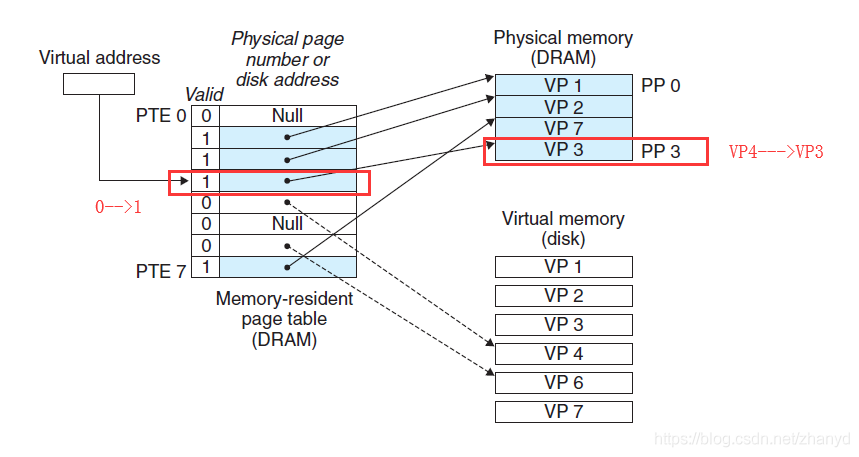
\includegraphics[width=0.7\linewidth]{figures/virtualMemory.png}
	\caption{virtualMemory}
	\label{fig:virtualMemory}
\end{figure}


\subsubsection{上下文信息}
进程上下文包括三个,用户及上下文,寄存器上下文和系统级上下文

用户级上下文:指令,数据,共享内存、用户栈

寄存器上下文:程序计数器,通用寄存器,控制寄存器,状态字寄存器,栈指针(用来指向用户栈或者内存栈)

系统级上下文:pcb(进程控制块),主存管理信息(页表\&段表)、核心栈

PCB:

表示进程的状态. 进程的优先级. pid 进程号

\subsubsection{内存访问}
TLB: 快表, 防止多级转换

MMU: 内存管理单元 将虚拟地址转为真实地址

虚拟地址: 页号+页内偏移; 可能产生多级页表: 一级页号+二级页号+业内偏移



物理地址: 硬盘上的地址


首先CPU先使用虚拟地址通过MMU转为真实地址, 查找TLB快表上是否有存储真实地址的值, 如果存在, 那么直接去拿到真实地址的值, 如果不存在那么: 虚拟地址第一级页号找到二级页表地址. 然后通过二级页好找到二级页表内的地址, 二级页表内存储了真实的物理页号, 找到物理页号+虚拟地址的偏移找到真实地址

\begin{figure}
	\centering
	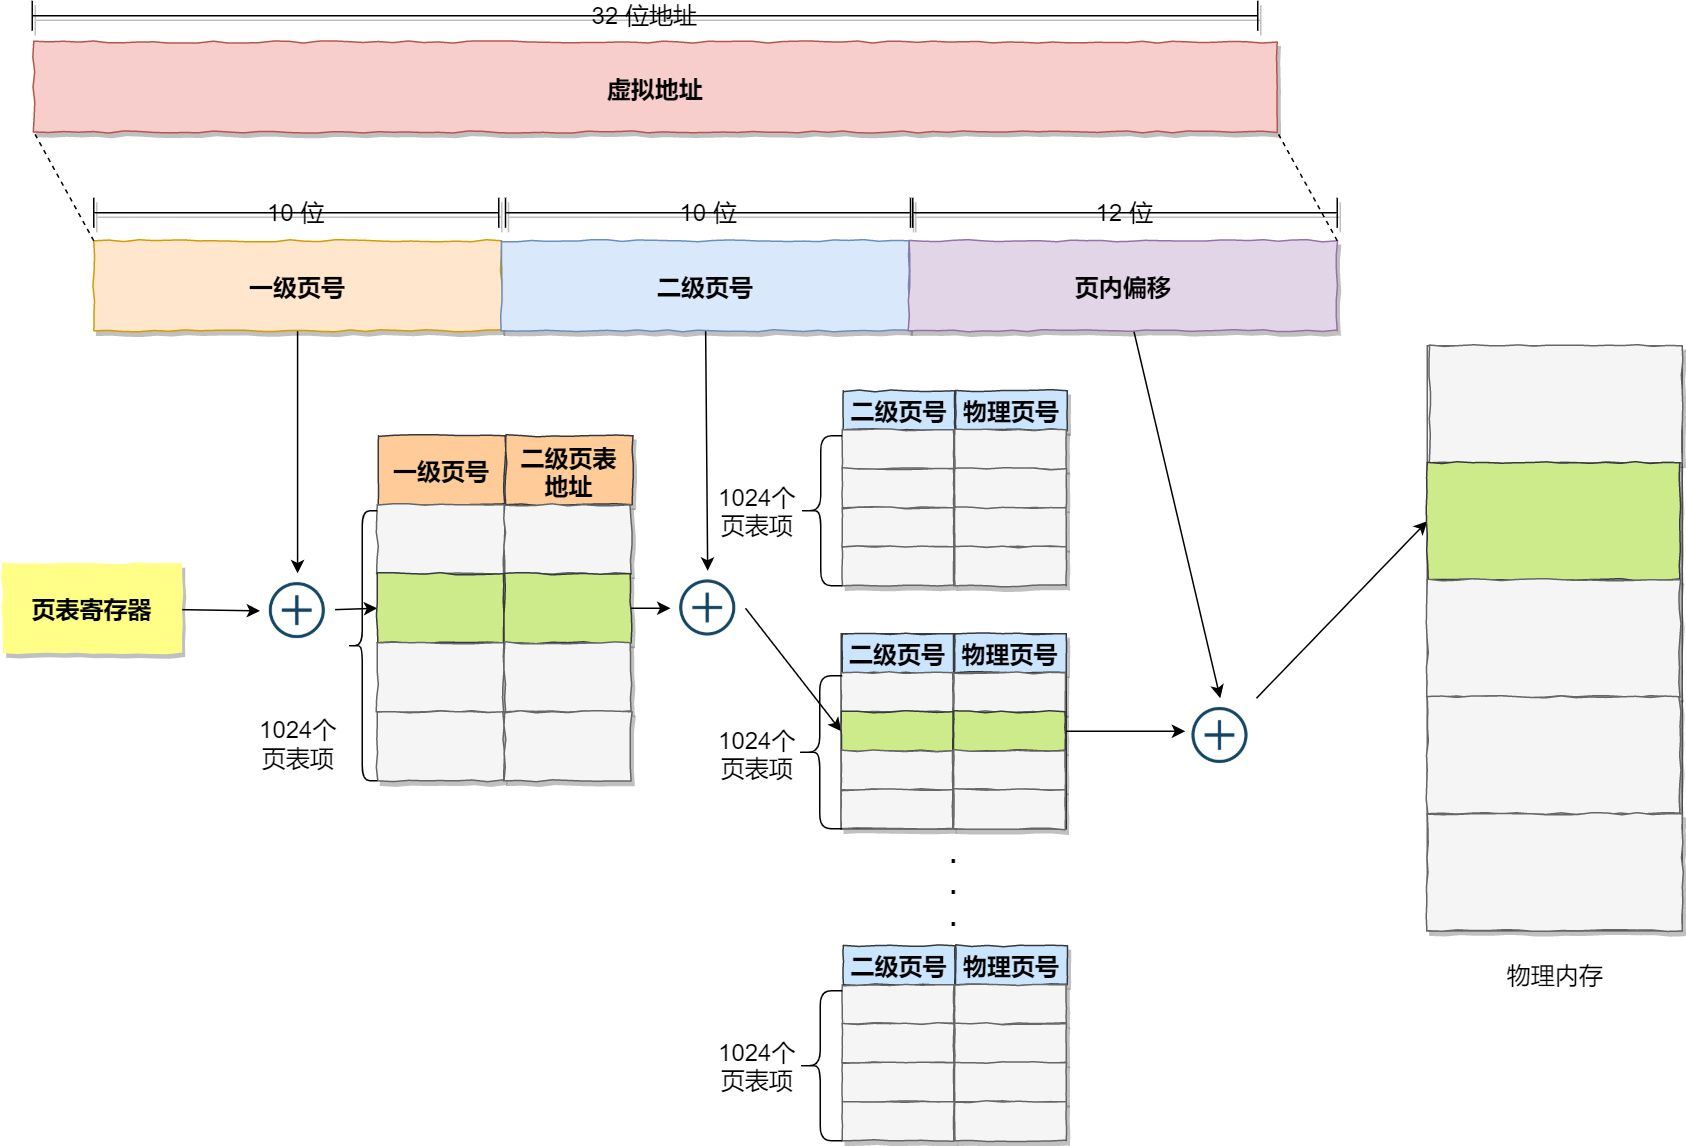
\includegraphics[width=0.7\linewidth]{figures/mmu.jpg}
	\caption{mmu}
	\label{fig:mmu}
\end{figure}

\subsubsection{匿名管道和命名管道的区别}
匿名管道由pipe函数创建并打开, 只能由父子进程进行半双工传递

命名管道由mkfifo函数创建,打开用open


\subsubsection{线程和进程的区别}
1. 一个线程从属于一个进程; 一个进程可以包含多个线程

2. 进程是系统资源调度的最小单位; 线程CPU调度的最小单位

3. 进程系统开销显著大于线程系统开销; 线程所需要的系统资源更少

4. 进程在执行时候拥有独立的内存尿胆原, 多个线程共享进程的内存, 如代码段, 数据段, 扩展端; 但每个线程拥有自己的栈段和寄存器组

5. 进程切换开销

a. 切换页表全局目录(比较费时, 对于大的进程之间的切换.)

b. 切换内核态堆栈

c. 切换硬件上下文

6. 线程切换开销

因为线程是进程的子集, 如果同一个进程之间的线程切换, 上下文会比进程切换要小.
\subsubsection{协程与线程进行比较}
协程, 是一种用户态的轻量级线程, 写成的调用完全由用户控制. 协程调度切换时, 将寄存器上下文和栈保存到其他地方, 在切回来的时候, 恢复先前保存的寄存器上下文和栈, 直接操作栈则\textbf{基本没有内核切换开销}, 可以不加锁访问全局变量. \par
(1) 一个线程可以有多个协程, 一个进程也可以单独拥有多个协程. \par
(2) 线程进程都是同步机制, 而协程则是异步 \par
\subsubsection{进程之间的通信方式有哪些?}
(1) 命名管道FIFO: 半双工方式 \par
(2) 消息队列: 克服了信号传递信息少, 管道只能承载无格式字节流以及缓冲区大小受限等缺点. \par
(3) 共享内存: 共享内存是最快的IPC方式. \par
(4) 信号量: 信号量是一个计数器. \par
(5) 套接字:socket 可以用于不同机器间的进程通信. \par
(6) 信号: 信号是一种比较复杂的通信方式, 用于通知接收进程某个事件已经发生, 比如linux中的kill命令通知进程进行关闭. \par
\subsubsection{进程调度算法}
(1) 先来先服务FCFS\par
(2) 短作业有限SJF \par
(3) 高优先权优先, 非抢占式优先权算法 \& 强占式优先权调度算法 \par
(4) 高响应比优先调度算法可以克服SJF长作业的饥饿 \par
(5) 基于时间片轮转调度算法 \par
\subsubsection{epoll和poll的区别}
1. select模型, 使用的是数组来存储Socket连接文件描述符, 容量是固定的, 需要通过轮询来判断是否发生了IO事件\par
2. poll模型, 使用的是链表来存储Socket连接文件描述符, 容量是不固定的, 同样需要通过轮询来判断是否发生了IO事件 \par
3. epoll模型, epoll和poll是完全不同的, epoll是一种事件通知模型, 大发生了IO事件时, 应用程序才进行IO操作, 不需要像poll模型那样主动去轮询 \par

select监控的句柄列表在用户态,每次调用都需要从用户态将句柄列表拷贝到内核态,但是epoll中句柄就是建立在内核中的,这样就减少了内核和用户态的拷贝,高效的原因之一。

还会再建立一个list链表,用于存储准备就绪的事件.

当epoll\_wait调用时,仅仅观察这个list链表里有没有数据即可。有数据就返回,没有数据就sleep,等到timeout时间到后即使链表没数据也返回。所以,epoll\_wait非常高效。
